\documentclass[DIV         = 16,
               fontsize    = 10,
               index       = totoc,
               landscape,
               twoside,
               headings    = small]{standalone}
\usepackage{tkz-euclide,tkzexample,pgfornament}
\usepackage{amsmath}
\usetikzlibrary{calc,fpu} 
\usetikzlibrary{math}

\tkzSetUpColors[background=white,text=darkgray]  
\tkzSetUpPoint[size=2,color=teal]
\tkzSetUpLine[ultra thin,color=teal]
\tkzSetUpCompass[color=orange,ultra thin,/tkzcompass/delta=10] 
\tikzset{label style/.append style={below,color=teal,font=\scriptsize}}
\tikzset{new/.style={color=orange,ultra thin}} 
\tikzset{step 1/.style={color=cyan,ultra thin}} 
\tikzset{step 2/.style={color=purple,ultra thin}}

\begin{document}

rlet{input}{red!80!black}
\colorlet{output}{red!70!black}
\colorlet{triangle}{orange!40}



\def\A{\textcolor{input}{$A$}}
\def\C{\textcolor{output}{$C$}}
\def\E{$E$}
\colorlet{triangle}{orange!80}
\colorlet{input}{red!80!black}
\def\B{\textcolor{input}{$B$}}
\def\D{$D$}

\begin{tkzexample}[vbox,small]
  \begin{tikzpicture}[thick,help lines/.style={thin,draw=black!50},old paper]
  \tkzDefPoint(0,0){A}
  \tkzDefPoint(1.25+rand(),0.25+rand()){B}
  \tkzInterCC(A,B)(B,A) \tkzGetPoints{C}{X}

  \tkzFillPolygon[triangle](A,B,C)
  \tkzDrawSegment[input](A,B)
  \tkzDrawSegments[red](A,C B,C)
  \tkzDrawCircles[help lines](A,B B,A)

  \tkzLabelPoints(A,B)
  \tkzLabelCircle[below=12pt](A,B)(180){$\mathcal{D}$}
  \tkzLabelCircle[above=12pt](B,A)(180){$\mathcal{E}$}
  \tkzLabelPoint[above,red](C){$C$}
  \tkzDrawPoints[fill=gray,opacity=.5](A,B,C)

  \tkzText[text width=8cm,align=justify](0,-4){%
     \small\textbf{Proposition I}\\
     \emph{To construct an \textcolor{triangle}{equilateral triangle}
     on a given \textcolor{input}{finite straight line}.}
     \\
       \vskip1em
     Let \A\B\ be the given \textcolor{input}{finite straight line}. \dots
  }
  \end{tikzpicture}
\end{tkzexample}

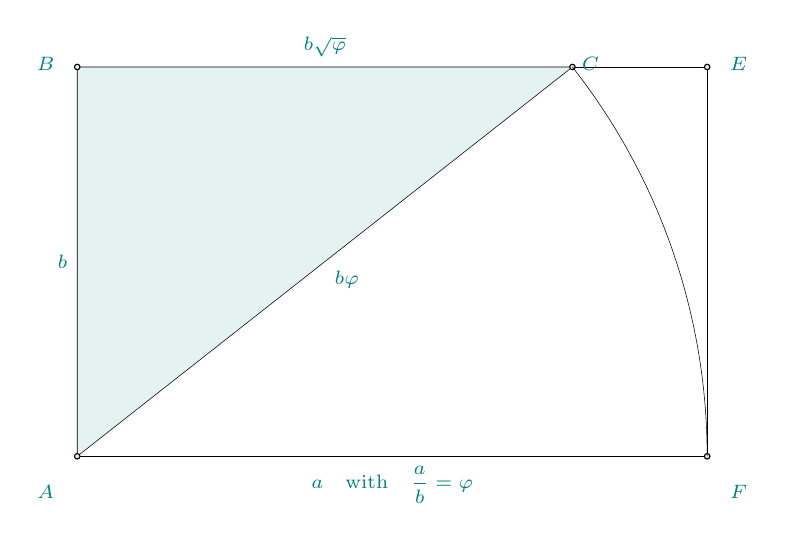
\begin{tikzpicture}[scale=1]
  \tkzDefPoint(0,0){A}   \tkzDefPoint(8,0){F}
  \tkzDefGoldRectangle(A,F)                       \tkzGetPoints{E}{B}
  \tkzDefBarycentricPoint(A=1,F=1,E=1,B=1)        \tkzGetPoint{w}
  \tkzInterLC[near](E,B)(A,F)                     \tkzGetFirstPoint{C}
  \tkzDrawPolygon(A,F,E,B)
  \tkzDrawPolygon[fill=teal!10](A,B,C)
  \tkzDrawPoints(A,B,E,F,C)
  \tkzAutoLabelPoints[center=w,dist=.1](A,B,E,F,C)
  \tkzDrawArc(A,F)(C)
  \tkzLabelSegment[left](A,B){$b$}
  \tkzLabelSegment[below right](A,C){$b\varphi$}
  \tkzLabelSegment[above](B,C){$b\sqrt{\varphi}$}
  \tkzLabelSegment[below](A,F){$a \quad \text{with} \quad \dfrac{a}{b}=\varphi$}
\end{tikzpicture}

\end{document}
